\documentclass{article}
\usepackage{graphicx}
\usepackage{amsmath}
\usepackage{amssymb}
\usepackage{amsfonts}
\usepackage{graphicx}
\usepackage{float}

\title{MEMAD-T05}
\author{ALEJANDRO ZARATE MACIAS}
\date{22 de Septiembre 2025}

\begin{document}

\maketitle

% ========================================
% INTRODUCCIÓN
% ========================================
\section*{Introducción}

% ========================================
% SECCIÓN 1
% ========================================
\section{Problema 1}

\subsection{Enunciado}

Considere la siguiente función
\begin{align*}
    f(x) = 2^{cos(x^2)}, \quad x \in (-\pi,\pi).
\end{align*}
A continuación, haga lo siguiente:

\begin{itemize}
    \item Calcule 500 pares de datos de muestra $D = {x_i,f(x_i)}$ donde los $x_i$ están equiespaciados.
    \item Realice un gráfico de $D$.
    \item Considere un modelo polinomial de grado $\mathcal{N}$:
        \begin{equation*}
            h(x_i, \theta) = \hat{y_i} = \sum^{\mathcal{N}}_{\ell=0}\theta_{\ell}x^{\ell}_{i}, \quad \theta=(\theta_{0}, \theta_{1}, \theta_{2}, ...,\theta_{\mathcal{N}}) \in \mathbb{R}^{\mathcal{N}+1}.
        \end{equation*}
    \item Considere una función de pérdida y costo de MSE:
        \begin{align*}
            Loss(y_i, \hat{y_i}) = (y_i - \hat{y_i})^2, \\
            Cost(\theta;D) = \frac{1}{m}\sum^{m}_{i=1}Loss(y_i, \hat{y_i})
        \end{align*}
    \item Codifique un script en Python para resolver el problema de optimización asociado utilizando un algoritmo de búsqueda lineal determinista. Puede probar $\mathcal{N}$ = 8, por ejemplo.
    \item Haz una gráfica de la solución contra $f(x_i)$ y muestra en otra gráfica cómo el costo disminuye a medida que pasan las iteraciones.
\end{itemize}

\subsection{Metodología}

Para resolver este problema, primero se deben implementar las funciones definidas en el enunciado ($f(x)$, $h$, $loss$ y $cost$).

Una vez implementadas estas funciones, procederemos a utilizar un algoritmo de búsqueda lineal determinista. Para este caso, emplearemos el método de Gauss-Newton implementado en tarea 04, pero ya con las correcciones realizadas en el algoritmo, a diferencia de la entrega pasada (en mi caso).

El procedimiento consistirá en:
\begin{enumerate}
    \item Generar 500 puntos equiespaciados en el intervalo $(-\pi, \pi)$ utilizando numpy y la función "linespace".
    \item Calcular los valores de $f(x_i)$ para cada punto.
    \item Aplicar el algoritmo de Gauss-Newton para encontrar los parámetros óptimos $\theta$.
    \item Finalmente graficar los resultados y el comportamiento de la función de costo.
\end{enumerate}

\subsection{Resultados}
\setcounter{equation}{0}

La Figura \ref{fig:fx} muestra la función original $f(x) = 2^{\cos(x^2)}$ evaluada en los 500 puntos de muestra equiespaciados en el intervalo $(-\pi, \pi)$.

\begin{figure}[H]
    \centering
    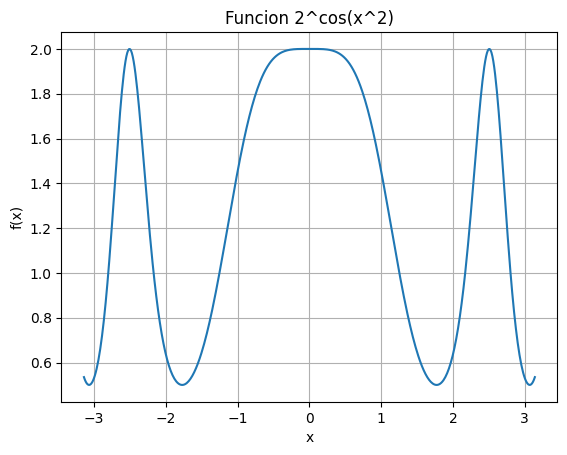
\includegraphics[width=0.8\textwidth]{images/1_fx.png}
    \caption{Función original $f(x) = 2^{\cos(x^2)}$ con 500 puntos de muestra}
    \label{fig:fx}
\end{figure}

Para los parámetros de optimización: $\mathcal{N}=8$, tasa de aprendizaje inicial $\alpha = 0.01$, 2000 iteraciones máximas y tolerancia de $1 \times 10^{-8}$, obtuvimos que el algoritmo de Gauss-Newton alcanzó su punto óptimo en 170 iteraciones.

\begin{figure}[H]
    \centering
    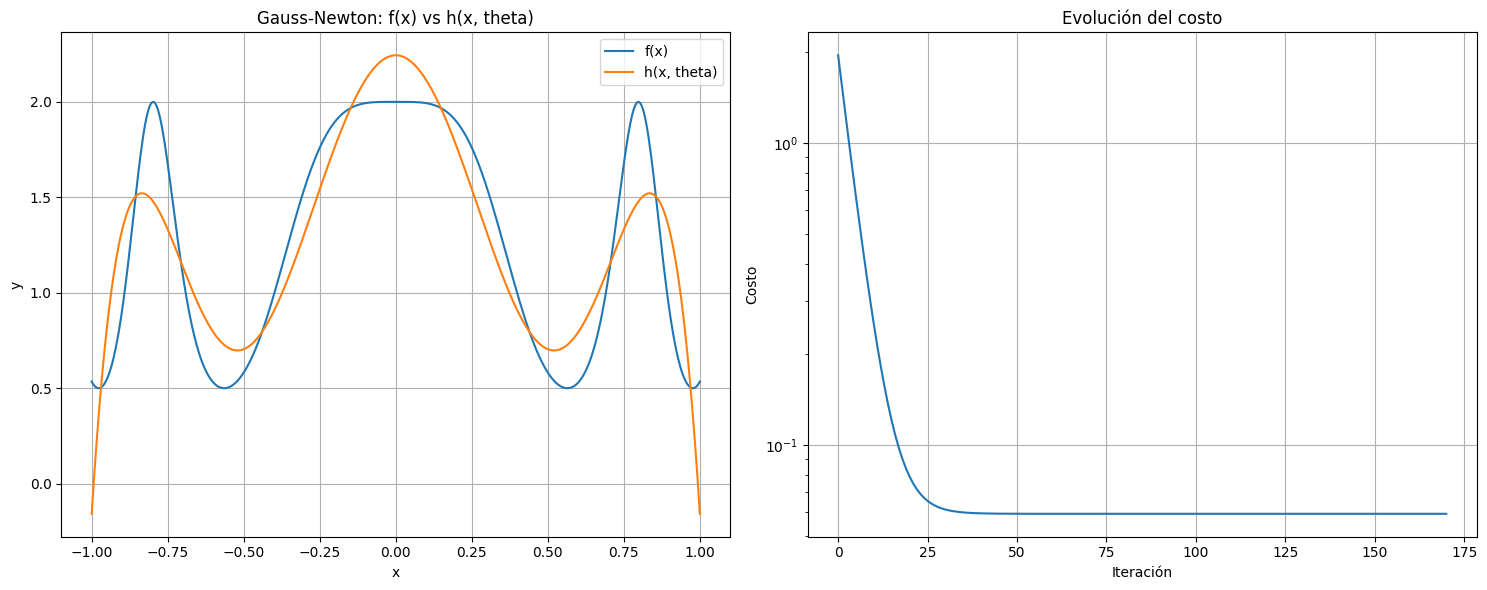
\includegraphics[width=0.8\textwidth]{images/1_gauss_newton_N8.png}
    \caption{Resultados del ajuste polinomial usando Gauss-Newton con $\mathcal{N}=8$}
    \label{fig:gauss_newton_results}
\end{figure}

\subsection{Discusión}

Después de haber podido implementar de manera exitosa el método de Gauss-Newton para esta tarea, a diferencia de la implementación pasada, logramos la convergencia de la función de manera satisfactoria. 

Para el caso del polinomio de grado $\mathcal{N}=8$, aunque la función resultante no hace un "fit" exacto a la función original, se asemeja considerablemente a ella. Esto es esperado dado que estamos aproximando una función con un polinomio de grado relativamente bajo a comparacion de la original ($f(x)$).

La convergencia en 170 iteraciones indica que el algoritmo fue eficiente para este problema particular, y la tolerancia establecida fue adecuada para obtener una solución de buena calidad.

\subsection{Conclusión}

Logramos resolver exitosamente el problema de optimización utilizando el método de Gauss-Newton. La implementación mejorada del algoritmo nos permitió obtener una convergencia adecuada y un ajuste polinomial que aproxima razonablemente bien la función objetivo $f(x) = 2^{\cos(x^2)}$. Los resultados demuestran que el enfoque determinista de búsqueda lineal es efectivo para este tipo de problemas de regresión polinomial, logrando una solución satisfactoria en un número bajo de iteraciones.


% ========================================
% SECCIÓN 2
% ========================================
\section{Problema 2}

\subsection{Enunciado}

Intenta encontrar un tamaño más adecuado para el modelo paramétrico del problema anterior resolviendo de nuevo varios valores de $\mathcal{N}$. Crea gráficos que muestren tus hallazgos. A partir de aquí, puedes fijar este valor de N para los problemas restantes.

\subsection{Metodología}

Para encontrar el tamaño más adecuado del modelo paramétrico, tomaremos la implementación previa del algoritmo de Gauss-Newton y procederemos a iterar con distintos valores de $\mathcal{N}$ para determinar cuál puede ser el más óptimo para este problema.

Después de varias pruebas experimentales, se descubrió que los puntos donde la función resultante llega a adquirir diferentes formas es con los valores $\mathcal{N} = [2, 4, 8, 12, 16, 20]$. Estos valores nos permitirán observar cómo evoluciona la aproximación polinomial conforme aumenta el grado.

El procedimiento consistirá en:
\begin{enumerate}
    \item Aplicar el algoritmo de Gauss-Newton para cada valor de $\mathcal{N}$
    \item Agrupar y mostrar las gráficas del resultado de la optimización de los valores $\theta$
    \item Comparar el avance del costo para cada grado de polinomio
\end{enumerate}

\subsection{Resultados}
\setcounter{equation}{0}

Para los valores de $\mathcal{N} = [2, 4, 8, 12, 16, 20]$ obtuvimos que casi todas las optimizaciones convergen en un número similar de iteraciones, pero los resultados son considerablemente distintos entre sí.

\begin{figure}[H]
    \centering
    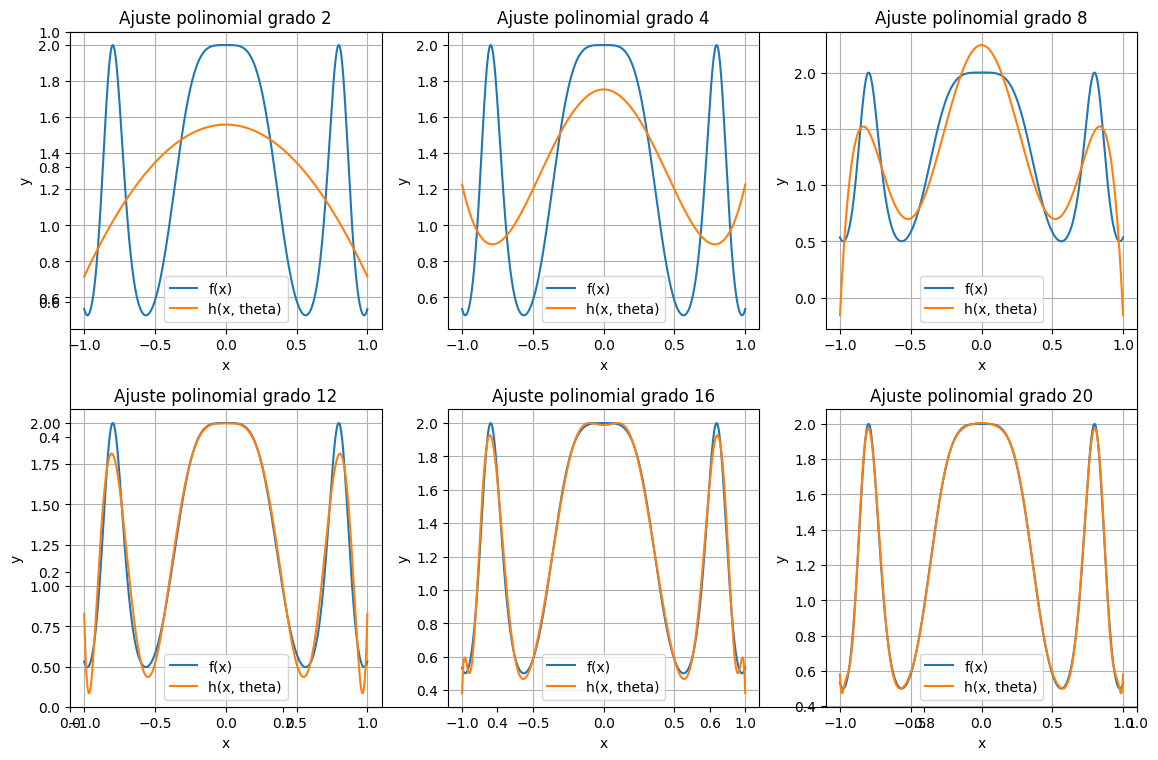
\includegraphics[width=0.8\textwidth]{images/2_comparasion_Ns.png}
    \caption{Comparación de ajustes polinomiales para diferentes grados $\mathcal{N}$}
    \label{fig:comparison_N}
\end{figure}

\begin{figure}[H]
    \centering
    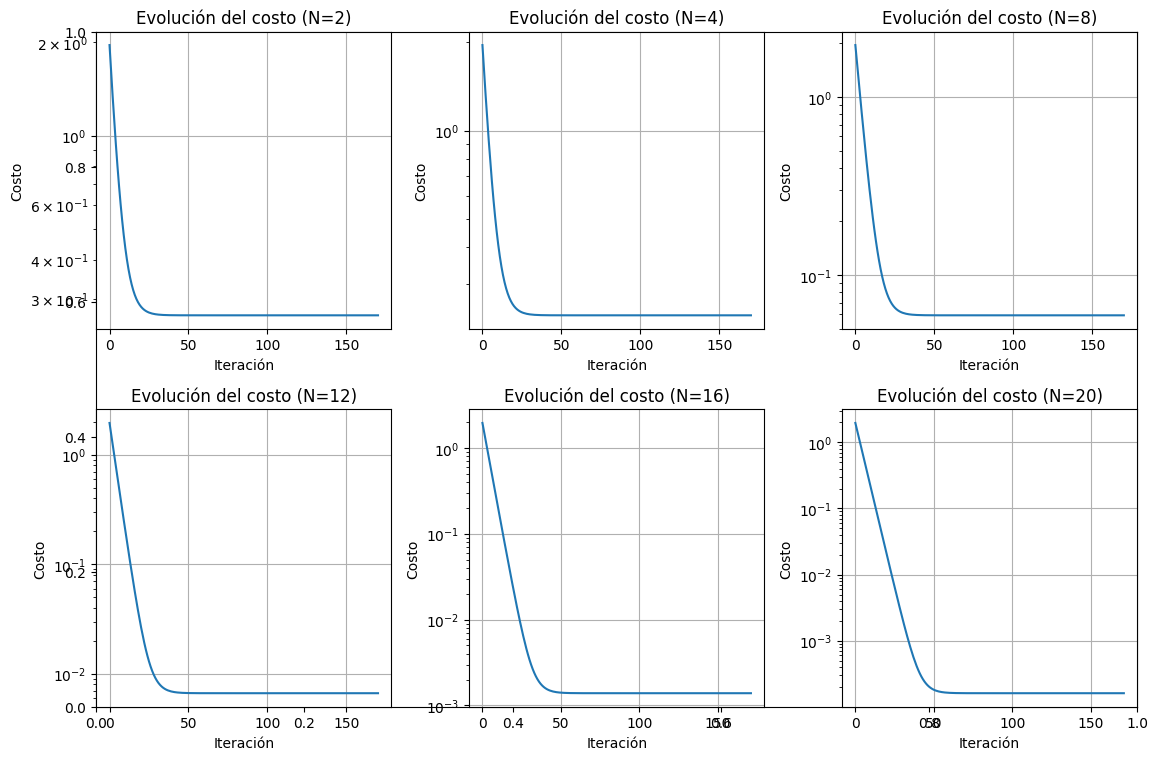
\includegraphics[width=0.8\textwidth]{images/2_comparasion_Ns_costs.png}
    \caption{Evolución del costo para diferentes grados de polinomio}
    \label{fig:comparison_costs}
\end{figure}

Los resultados muestran que conforme aumenta el grado del polinomio, la aproximación a la función original mejora significativamente, especialmente para $\mathcal{N} \geq 12$.

\subsection{Discusión}

Pese a que $\mathcal{N} = 20$ resultó ser el valor más apegado a la función original, es considerablemente más costoso computacionalmente calcularlo. Por el contrario, $\mathcal{N} = 12$ representa un polinomio no tan grande pero con una aproximación bastante decente.

Los polinomios de grado bajo ($\mathcal{N} = 2, 4$) muestran aproximaciones muy limitadas que no capturan la complejidad de la función original. Los grados intermedios ($\mathcal{N} = 8, 12$) ofrecen un buen balance entre precisión y eficiencia computacional, mientras que los grados altos ($\mathcal{N} = 16, 20$) proporcionan la mejor aproximación a costa de mayor complejidad.

\subsection{Conclusión}

Logramos identificar que $\mathcal{N} = 12$ representa el valor óptimo para el modelo paramétrico, ofreciendo un equilibrio adecuado entre precisión de aproximación y eficiencia computacional. Este valor será utilizado en los problemas restantes, ya que proporciona una aproximación satisfactoria de la función original sin el costo computacional excesivo de polinomios de mayor grado. Los resultados demuestran la importancia de evaluar múltiples grados para encontrar el balance óptimo entre complejidad del modelo y calidad del ajuste.

% ========================================
% SECCIÓN 3
% ========================================
\section{Problema 3}

\subsection{Enunciado}

Cree un script para resolver el Problema 1 utilizando un gradiente descendente de Minibach con una tasa de aprendizaje constante $\alpha$. Genere una gráfica de la solución en función de $f(x_i)$ y muestre en otra gráfica cómo disminuye el coste a medida que transcurren las iteraciones.

\subsection{Metodología}

\subsection{Resultados}
\setcounter{equation}{0}

\subsection{Discusión}

\subsection{Conclusión}

% ========================================
% SECCIÓN 4
% ========================================
\section{Problema 4}

\subsection{Enunciado}

Repita el Problema 3 usando Adam.

\subsection{Metodología}

\subsection{Resultados}
\setcounter{equation}{0}

\subsection{Discusión}

\subsection{Conclusión}

% ========================================
% SECCIÓN 5
% ========================================
\section{Problema 5}

\subsection{Enunciado}

Compara las soluciones y el rendimiento de los tres algoritmos que utilizaste para resolver el problema 1. Escribe tus conclusiones y haz algunos gráficos.

\subsection{Metodología}

\subsection{Resultados}
\setcounter{equation}{0}

\subsection{Discusión}

\subsection{Conclusión}

% ========================================
% SECCIÓN 6
% ========================================
\section{Problema 6}

\subsection{Enunciado}

Hasta ahora has resuelto un problema sin ruido, es decir,

\begin{equation*}
    f(x)=2^{cos(x^2)}+\mathcal{X}, \quad x \in (-\pi,\pi), \mathcal{X} \sim \mathcal{N}(0,\sigma^{2}),
\end{equation*}

Donde solo se ha considerado el caso con $\sigma^2=0$. Repita los ejercicios 1 a 5 para los niveles de ruido $\sigma^2 = 0.05,0.1,0.5$. No olvide anotar todas sus conclusiones y reflexiones.

\subsection{Metodología}

\subsection{Resultados}
\setcounter{equation}{0}

\subsection{Discusión}

\subsection{Conclusión}

% ========================================
% SECCIÓN 7
% ========================================
\section{Problema 7}

\subsection{Enunciado}

Explique con sus propias palabras lo siguiente:

\begin{itemize}
    \item[(a)] Las diferencias y similitudes entre el descenso de gradiente estocástico, el descenso más pronunciado y el descenso de gradiente en minilotes.
    \item[(b)] Algunos ejemplos del uso de los tres últimos algoritmos citados (es decir, explique cómo identificar cuándo se debe utilizar un algoritmo entre otros).
    \item[(c)] Algunos ejemplos del uso de un enfoque determinista (Newton, descenso más pronunciado, BFGS, Gauss-Newton, etc.) y un enfoque estocástico (descenso de gradiente estocástico, descenso de gradiente en minilotes, Adam, etc.), es decir, explique cómo identificar cuándo se debe utilizar un enfoque particular sobre otro.

\end{itemize}

\subsection{Metodología}

\subsection{Resultados}
\setcounter{equation}{0}

\subsection{Discusión}

\subsection{Conclusión}

\end{document}
